%!TEX root = main.tex
\chapter{Peaceful Banana - An overview}
\label{peacefulBananaApplication}
In this chapter we will introduce the PeacefulBanana tool, which is the prototype we developed for our thesis. The purpose of this chapter is to explain the concept of the tool, it's features and the functionality it provides. The tool will be presented at a high-level, as the process of how we developed the prototype, design choices and implementation is further described in Chapter \ref{chap:design} \& \ref{chap:implementation}.
\section{What is PeacefulBanana?}
Peaceful Banana is a tool aimed towards aiding reflection in software development teams. It integrates with version control systems(VCS)\footnote{Version control is the management of changes to documents, computer programs, large web sites, and other collections of information}, which is commonly used in software development. The PeacefulBanana tool collects project artifacts from such version control systems and scaffolds these in order to trigger and promote reflection in teams. PeacefulBanana integrates with VCS and provides a layer of features specific for aiding reflection in software development projects. I.e.  PeacefulBanana will not feature the same functionalities that already exists in these systems, but rather contextualize them and present the data in a manner that can help teams reflect on their experiences. The tool will collect different data relevant for reflection, e.g. prompting the user for their mood each day, which allows for both team-wide and personal mood-graphs over a period of time. \\
PeacefulBanana is developed as a web-application and will work in all modern web-browsers running on platforms like PCs/MAC, smartphones and tablets.
The tool was developed with project artifacts collected from VCS in mind. The PeacefulBanana tool is developed for use in software development teams that have adopted an agile process model. Most agile process models feature reflection sessions in some form, in which this tool is used in order to promote and enhance the reflection that takes place in these sessions. Although it is aimed at agile teams, any process model featuring some kind of reflection session could benefit from using this tool. Similarly the tool can also be used individually at any time as a more general project overview tool. \\
The goal of PeacefulBanana is to present software development teams with a tool that can help them collect, revisit and reflect upon their experiences in both an individual and collaborative setting. Through the process of developing the prototype, it has become a tool that also supports collection of project artifacts and the presentation of these to users, in order to promote and trigger reflection. 

\section{What does it do?}
\label{whatdoesitdo}
PeacefulBanana is a tool that allows users to reflect upon and share their individual and collaborative experiences from development projects. The tool focuses on collecting project artifacts from VCS like code commits, milestones and issues as well as comments and references. The tool then scaffolds these data and presents them to the users, acting as input for users to revisit experiences and trigger reflection upon these. The reflection that occurs will be captured and stored as reflection notes so the user can review these at a later date. These notes, containing a user's reflection around that day's work experiences, can also be shared with the team and used by the user's team in reflection sessions. The tool is in this way designed to support both individual and collaborative reflection around work experiences. It can be used during the team reflection workshop or just browsed individually when the user wishes to. The tool provides several opportunities to the users:
\begin{description}
	\item[Provide a scaffolded overview of the project] \hfill \\
	PeacefulBanana provides users and teams with an overview of the project:
	\begin{itemize}
		\item Users can choose what team-project to retrieve data from, see the projects milestones, issues and generate data relevant for reflection from these.
		\item The team can see when an issue has been closed, and what milestones they are connected to.
		\item The team can see which milestones were closed and when, and easily see if the team met their deadlines. 
		\item The team can see which team members have contributed to which parts of the project.
	\end{itemize}

	\item[Individual 5-minute daily reflection] \hfill \\
	Each day a notification will prompt the user to perform a daily 5-minute reflection. This daily reflection note presents the user with data for the last 24 hours, i.e. project activity and a tag cloud. This data provides the user with additional information and tries to trigger reflection in the users based on that day's experiences The reflection note collects input from the user:
	\begin{itemize}
		\item The user's mood that particular day, ranging 5 steps from 0 (Very sad) to 100 (Very happy)
		\item The top 2 contributions done by the user in the project that day.
		\item The top 2 fields the user can improve on in the project.
	\end{itemize}
	Figure \ref{dailynote2} shows how the daily reflection note looks in the PeacefulBanana application
		\begin{figure}[!htpb]
		\centering
		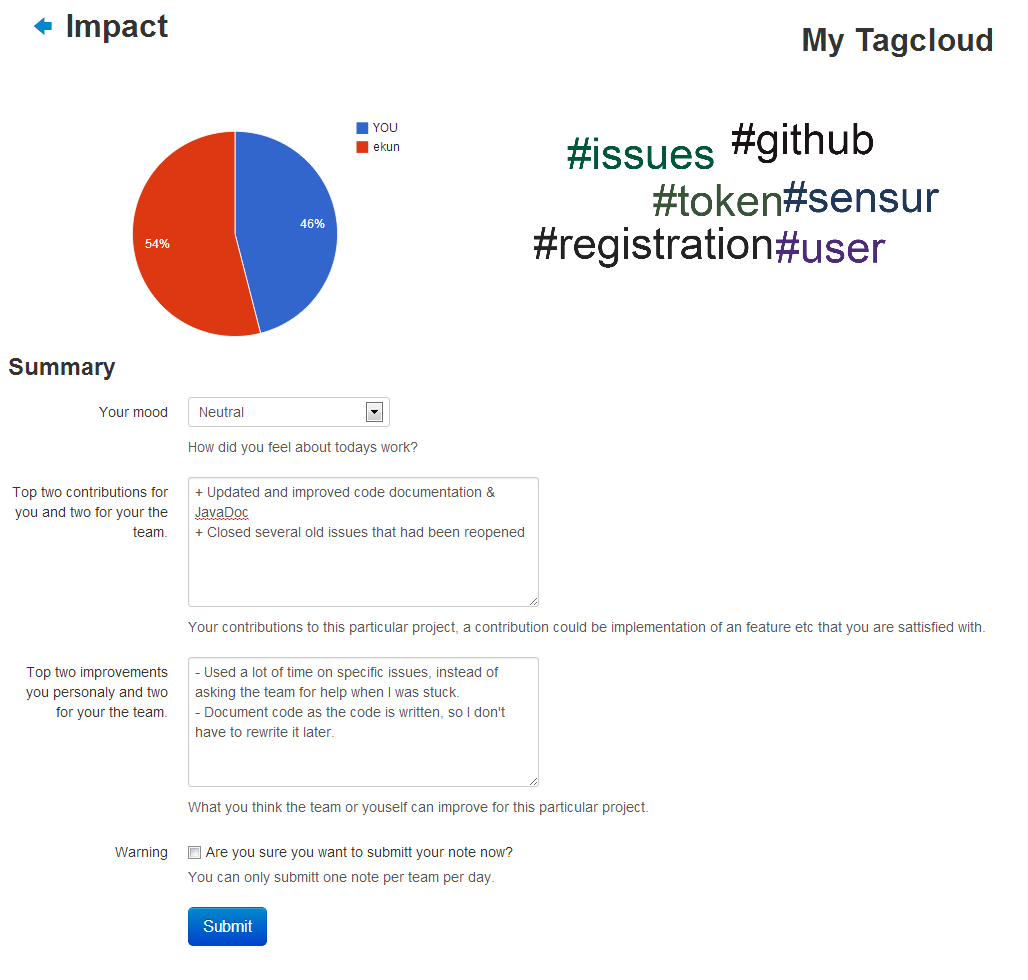
\includegraphics[width=\textwidth]{dailynote}
		\caption{PeacefulBanana Daily reflection note}
		\label{dailynote2}
	\end{figure}
	The PeacefulBanana application stores each of these daily summaries in a secure database. Each reflection note can also be shared with the user's team, but sharing notes is not required. The mood data collected each day is used by the application to generate a team-wide mood-average graph. This graph can be used to trigger a discussion and reflection in the team reflection sessions. 

	\item[Reflection sessions] \hfill \\
	The team, or the team leader can create a workshop from a selected time-period. The workshop presents some mandatory questions
	related to team work and reflection. Additionally the team can choose a set of tags to generate questions from. The finished workshop template can be printed and handed out to the team at the workshop, providing project statistics, trending issues, tag clouds and questions that act as reflection triggers\\
	Examples of such questions: 
		\begin{itemize}
			\item What were your initial expectations to this iteration? Did these expectations change during the iteration? How? Why?
			\item What could be done to improve team collaboration?
			\item Talk about any disappointments or successes of your project. What did you learn from it?
			\item You have had a high activity working with \#framework Did you experience any particular problems with this tag? Why or why not?
			\item What did you learn from working with the issue \textit{daily summary \& reflection notes (\#17)}?
			\item The team didn't meet the deadline for milestone \#20 - Midterm Report, did the team experience any particular problems?
		\end{itemize}
\end{description}
Figure \ref{workshopquestionspeaceful} shows an example of a project workshop and the questions generated for it based on the project tags. 
	\begin{figure}[!htpb]
		\centering
		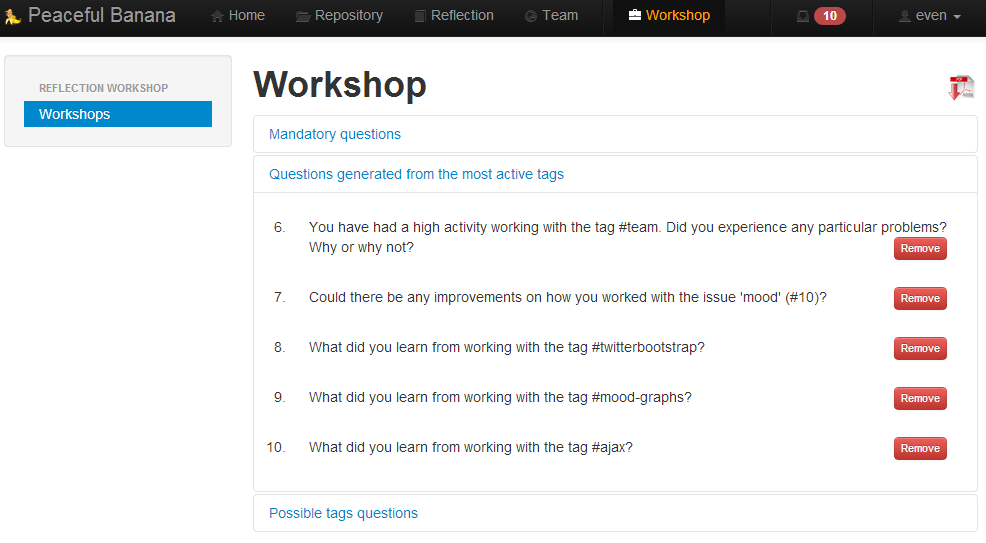
\includegraphics[width=\textwidth]{workshopgenerated}
		\caption{PeacefulBanana Reflection Workshop - Generated Questions based on project tags}
		\label{workshopquestionspeaceful}
	\end{figure}